\chapter{Modulation of SWR incidence}

  In this chapter I introduce the in-vitro SWR model. I survey the literature
  on different drugs that modulate the incidence and other properties of the
  SWs. I present some analysis of in-vitro data provided by Nikolaus, where
  slices were infused with gabaA antagonist gabazine and gB antagonist SCH..

\section{Summary}

  Sharp-wave ripples are network events in the hippocampus that involve large
  number of cells that fire in synchrony within a time window of 20-100 ms.
  Despite the huge attention that SWRs are attracting, the exact mechanisms of SW
  generation, termination are still debatable.  An in-vitro model of SWs was
  developed by Maierxxxx has largely facilited the study of the SWs. In this
  chapter I review the literature on the effects of various drugs on the SW
  incidence and discuss on the possible mechanisms of drug control on SWs.
  Moreover, I analyse 2 datasets of in-vitro recordings provided by Nikolaus and
  show that the gaabaA antagonist gabazine does not only decrease SW incidence
  but also increases SW amplitudes. GabaB antagonist SCH..., on th eother side
  increases SW incidence but decreases the amplitude of the events. The results
  suggest the existance of a limited resourse that is gettting depleted by SWs
  and recovered by time


\section{Introduction}

  \subsection{SWRs in vitro}
    tao: read Chap from Richard and Nikolaus; and Buzsaki review on in-vitro models!
    chamber and interface???
    occur in tiniest slice, comparison with in vivo swrs; mini slices..

  \subsection{Modulation of SWRs}
    The exact mechanisms of SW generation, and modulation in general, are still
    elusive. What controls the rate of SW occurrence, their length, or
    amplitude. How are they terminated, and why does their duration is
    relatively constant? What is the mechanism behind the fast ripple
    oscillation, and what is its function? A large amount of work has been put
    to answer the questions above. For some the problems, there is general
    agreement, for others less. To shed some light on the progress of cracking
    the SWRs, in this section I review the literature on SWs, and in particular
    the studies that have studied how do the SWs properties change under the
    influence of various drugs..

    motivate a bit better, Sw are network phgenomenon, way to study is to manipulate various parts of this network. drugs are good tool. specific...here ,mostly focus on inh modl drugs: gabazine, BZL, steroids, GB blockers, GIRK blockers...

    gaba is most ubiqulous inhibitory neurotransmitter? blabla
    gabaR: A and B
    ambient gaba; how to measure

    \subsubsection{Exciting a single PC cell}

      - Maja: single PC stimulation leads to SWs

    \subsubsection{Exciting a single PVBC cell}
      - PV+IN stim leads to SWs


    \subsubsection{GABAaR}
      gabaARs: types; subunits, locations....

      gabazine, BCL, steroids...?
      - Nimmrich2005: 0.3 uM gabazine decreases incidence and slowly abolished SWRs; more gabazine -> faster abolishment
      - Maier2003: 3uM gabazine blocks totally SWs 

      Bicuculline: a light-sensitive competitive antagonist of GABAA receptors blocks both tonic and phasic GABAa receptors


    \subsubsection{GABABR}
      gabaBRs: types; subunits, locations....

      GIRK blockers, gB antagonists...

    \subsubsection{Exc R modulation}
      CNQX: ampa/kainate receptor antagonist: 20uM blocks SWRs (Maier2003)

    \subsubsection{Canabinoid R}
      Maier2012:
          CB1 most ubiquitous G protein-coupled neuromodulatory receptor (Maier 2012); experssed presynaptically on CCK+ IN; glut terminals on pyramids in CA1
      CB1 receptor agonist: 1uM CP55,940 decreases SW incidence.
      CB1 receptor agonist: 1uM WIN55,212-2 decreases SW incidence.
      CB1R antagonist blocks AM251 the effect of WIN-2; no change in incid or ripples when AM only
      20uM $\Delta^9 \rm -THC$ also decreased SWR incidence but took longer to take action and more
      block of endocannabinoid-degrading enzymes had no effect on SW incid.

      adenosine: activates GIRK channels, decreases input resistance and hyperpolarises neurons.
        - presynaptic modulation of exc transmitter release; regulates gabazine (Wu and Saggau1994; Gundlfinger07)
        - 10uM adenosine decrease SWR incidence comparable with 1uM WIN-2
        - GIRK channel blocker and adenosine the same effect as only adenosine; ruling out postsynaptic (GIRK) effects

    \subsubsection{Electrical coupling}
      roger, roger...
      

\section{Methods}
  
  This chapter is mostly based on the analysis of data provided by Nikolaus
  Maier from Schmitzlab. Here, I analyse 4 (and a half) datasets of {\it in vitro}
  recordings. All the recordings were performed in the CA3 area of hippocampal
  slices. Here we give a brief summary about the datasets and provide some
  details on the applied techniques during their analysis.

  The simulation results are based on the model described in Chapter
  \ref{ass_sequences}....

  in hp there are over 20? types of INs. in this chapter when we infer to
  IN, we mean a hypothetical neurons that are active outside the SWs and keep
  the network into balance state. Candidate cells for for this role are...


  \subsection{Data}
  %___________________
  
    \subsubsection{Dataset 1: gabazine}
     
      8 recordings.
      extracellular field potential, a few tens of minutes after the beginning of recording gabazine is infused in the extracellular solution.
      Sampling rates are between 5 and 10 kHz.
      Multiple sweeps of 30/60 seconds.
      In two recordings there was washout of the gabazine.
      gabazine 


      for further analysis time windows were chosen for the comparisons:
        -12 , -3 before and 6, 11 after the drug infusion.
        time to go home!

    \subsubsection{Dataset 2: SCH50,911}
      The second dataset contains extracellular recordings from 13 slices.
      Here, extracellular field potential is measured for several minutes
      depending on the recording, and later on the drug SCH50,911 was infused
      into the ?solution.  SCH50,911 is a ${\rm GABA_B}$ receptor antagonist
      which acts on presynaptic as well as on postsynaptic receptors.


    \subsubsection{Dataset 3: Extra and Intra}
      The third dataset consists of 13 pairs of recordings.  Each pair contains
      simultaneous extracellular field recording and intracellular recording
      from a patched pyramidal cell in a current clamp mode.  The recordings
      consist of multiple sweeps of around 5-20 seconds.  The length of each
      recording is rather short, ranging from 40 seconds up to 10 minutes.  The
      sampling rates are between 5 and 40 kHz.

  \subsection{Data analysis}
    \subsubsection{SWR detection}
      For the detection of SWRs, the extracellular LFP signal is used. The raw
      signal, typically in 5-20kHz sampling rate, is band-passed filtered in
      the range 2-50? Hz. Some recordings that showed oscillatory component in
      the 3.3 Hz frequency were filtered in the range 4-50Hz.... 

    The SWR events are detected in the extracellular recordings.
    The traces are filtered in the frequency band of 5-60 Hz??.
    Then SWRs are detected whenever the filtered signal crosses a defined threshold which was set for each recording individually.
    The thresholds are set in terms of standard deviations, typically 2-4 SDs.

    however, data is often noisy, and not all SWs are detected correctly.
    For example in number of recordings it was difficult to set up an appropriate threshold as there are some small field events that a pretty much indistinguishable from the SWRs but with very small amplitudes, and any reasonable threshold would leave them out as non-events. This suggests that in some experiments the SWRs are not all-or-none events but they have very continuous distributions of sizes.

    few comments on ripples and data quality...
    Example figure of raw and filtered trace, maybe intracellular recording as well...
    of clean and tidy recording and another of a mess..

    In the last dataset (MEA), the data was preprocessed and SW events were detected in all the electrodes.
    What I did is only to take the peaks of the already detected SWs in the raw data and correlate them across electrodes to see if a large SW at one location implies a large event at another location.
    
\section{Results}
%___________________

  Here I present the main results from the data analysis and speculate about
  possible mechanisms underlying the occurrence of SWRs. explore a few hypothesis and etc.

  \subsection{Gabazine decreases SWR incidence {\textit {in vitro}} }
    Gabazine is a drug that blocks phasic $\rm GABA_A$ receptors, effectively decreasing the
    inhibitory conductances. So it is intuitive to expect a more excited
    network. However, it has been shown refs??  that application of gabazine
    decreases the number of SW occurring spontaneously. Can we explain that?  In
    this section I analyse a few recordings performed by Nikolaus where
    gabazine was applied in hp slices.

    \begin{figure}
      \includegraphics[width =35pc]{4feb14_slice1.png}
      \caption{Example of a recording with gabazine infused into the extracellular solution?
                Gabazine decreases the SWR incidence.
             }
      \label{fig:gabazine_ex}
    \end{figure}

    In Figure \ref{fig:gabazine_ex} is shown an example recording where
    extracellular field potential is measured in CA3 of hippocampal slices.
    Average incidence ($\#$ events/second) is plotted in time in 1 minute time
    resolution. After 41 mins of baseline recording, 100 uM of gaabzine was
    infused into the extracellular solution (denoted with a horizontal red
    line). Incidence goes down.. SW peak and duration are relatively stable
    over the whole recording (second to forth subplot).

    Overlying all SW detected (before and during drug) relatively to the
    filtered peak of the SW shows rather stereotypical SW waveform where even
    the ripples are alligned as seen in the black trace. The individual traces
    are plotted in gray lines while the average is shown in black (bottom row,
    left and middle columns). Mean SW waveform is not affeted by the gaabzine
    application (bottom right plot).  I note that this is the most prominent
    example with the ripple being preserved after averaging.


    \begin{figure}
      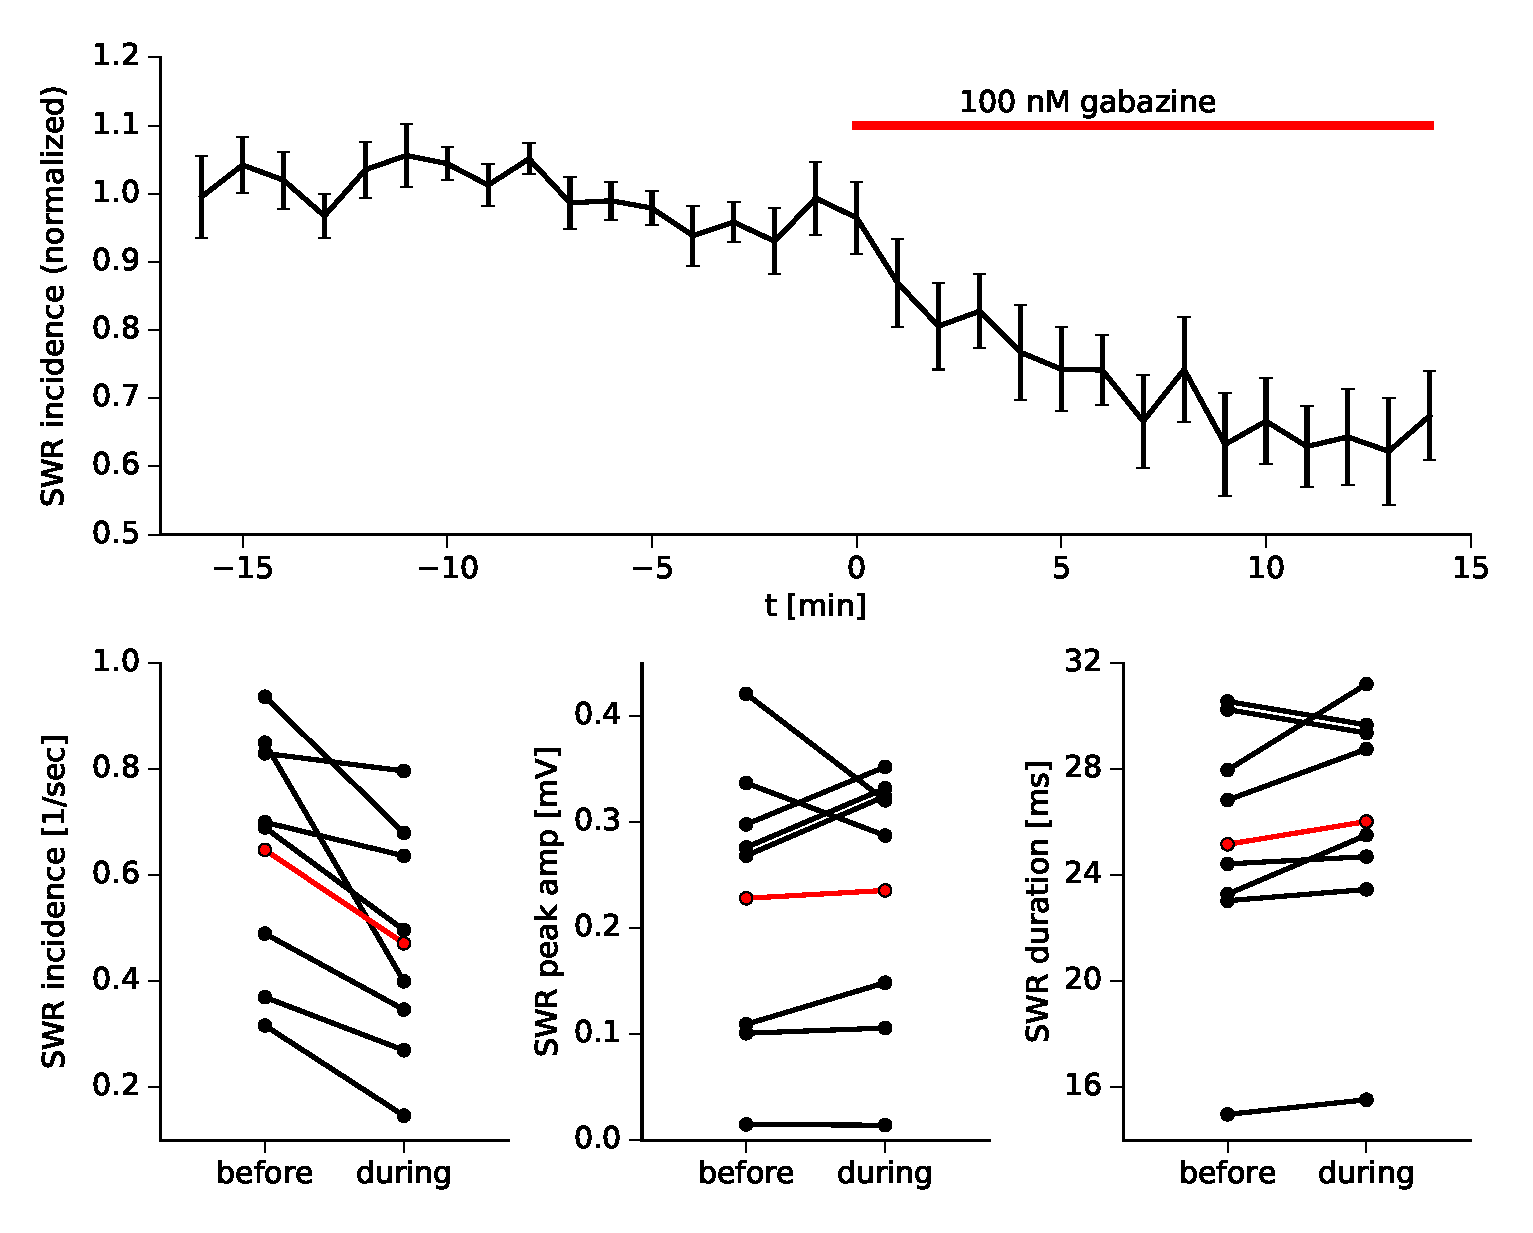
\includegraphics[width =35pc]{gabazine_events_all.eps}
      \caption{Gabazine decreases the SWR incidence. Pooled data from 8 recordings..}
      \label{fig:gabazine_sum}
    \end{figure}

    gabzine decreased the incidence in 7 from 8 recordings. The avergae effect
    is shown in Figure \ref{fig:gabazine_sum} where the incidence is normalized
    relative to the incidence before drug application. Gabazine starts
    affecting the incidince alreeady 1 minute after application and takes
    around 5 mins to take full effect.

    To characterize drug effects on SWs I analyse the events in constarained
    time window only. Events in the window [-7, -2] mins and [6, 11] mins
    were used to calculate properties of SWs before and after the drug,
    respectively (Figure \ref{fig:gabazine_sum} bottom row). As mentioned
    before there is a strong effect on the incidence, however, somewhat weaker
    effects are observed on the SW peak and SW duration. While SW tend to get
    bigger after gabazine applicagtion, i.e., to have larger peak and to last
    longer. Update that all show decrease in incidence, amplitude increase is
    less prominent. but also very dependent on the window..usually it increases
    more.

    This finding is in odds with Schlingloff2014 who showed that a local puff
    of gabazine decreases locally the SWR amplitude.  In the slices used for
    this analysis, however, the global infusion of gabazine slightly increases
    the SWR amplitude.  The incidence in Schilingloff is, however, intact as
    SWRs occur at other locations of the slice.  An explanation could be that
    the after gabazine the tissue needs longer time to recover after an event,
    which is the case in our slices. In Schiligloff after the locall gabazine
    puff, however, SWs occur all the slices and propagate to the area that is
    affected by the drug and in we see only their shadow...

    \begin{figure}
      \includegraphics[width =35pc]{Schlingloff_3bcd5e.png}
      \caption{local application of Gabazine decreases amplitude, spikes (b,c,
        and d from thir Fig3), increases PVBC firing (e from their Fig 5)
            }
      \label{fig:schlingloff_gabazine}
    \end{figure}

    Local gabazine puff decreases the SW peaks in Schilinglof, but is also
    decreases the MU firing \ref{fig:schlingloff_gabazine}. Cells are more
    inhibited? However in another experiment the same authors measured PVBCs in
    a loose patch and show that their FR is increased. This suggests some
    disinhibitory mechanisms.... pc/PVBC ratio is 95/5 or 98/2...
    
    In summary, PC seems to be less excitable (due to lower FRs), while PVBCs
    fire more when gabazine is applied. Paradox: how does it happen that
    decreasing inhibition decreases SWR incidence, i.e., the network gets less
    excitable or more inhibited?  Next section will deal with that question in
    a modelled network where I explore some effects of decreased inhib
    conductances.

    Possible GBr receptor activation???? higher IN activity, leads to more
    gaba, more extrasynaptic activations...then 

  \subsection{Gabazine influence on SWR incidence {\textit {in silico} }}

    To better grasp the behaviour of the network under gabazine influence I use
    the numerical network presented in the previous chapter as a model for the
    spontaneously occurring SWs and a linear Firing model.

    In the simulations presented here, the same parameters values from from the
    previous chapter are used (see materials and methods).  Briefly, I embedded
    sequences of neural assemblies consisting of both e AND I neurons into a
    randomly connected network. Recurrent connectivity (pr=0.08) describes the
    connection proabability within assembly while the feedforward connectivity
    (pf=0.06) is the connectivity between E neurons of consequent assemblies in
    the sequence. Using these parameters allows noise flactuations in the FRs
    to get amplified by th eff structure of the sequence resulting in
    spontaneous replays (ref fig spont repl).
    This is illustrated in the rsater plot (fig ) of E neurons, whwre the black
    dots show individual spikes, and the stripes are burst of synchronous
    activity. To model the gabazine effects, here the network is balanced. at
    time 21 sec gabzine infusion is modelled by decreasing all inhib
    conductances with 90-95\% of their initial value. As intuitively expected
    this decreases the total inhib of the network resulting in higher Frs and
    more freqeunt spont bursts. This result is in direct collision with th e
    gabazine effects that are reported in in-vitro studies (refs).

    \begin{figure}
      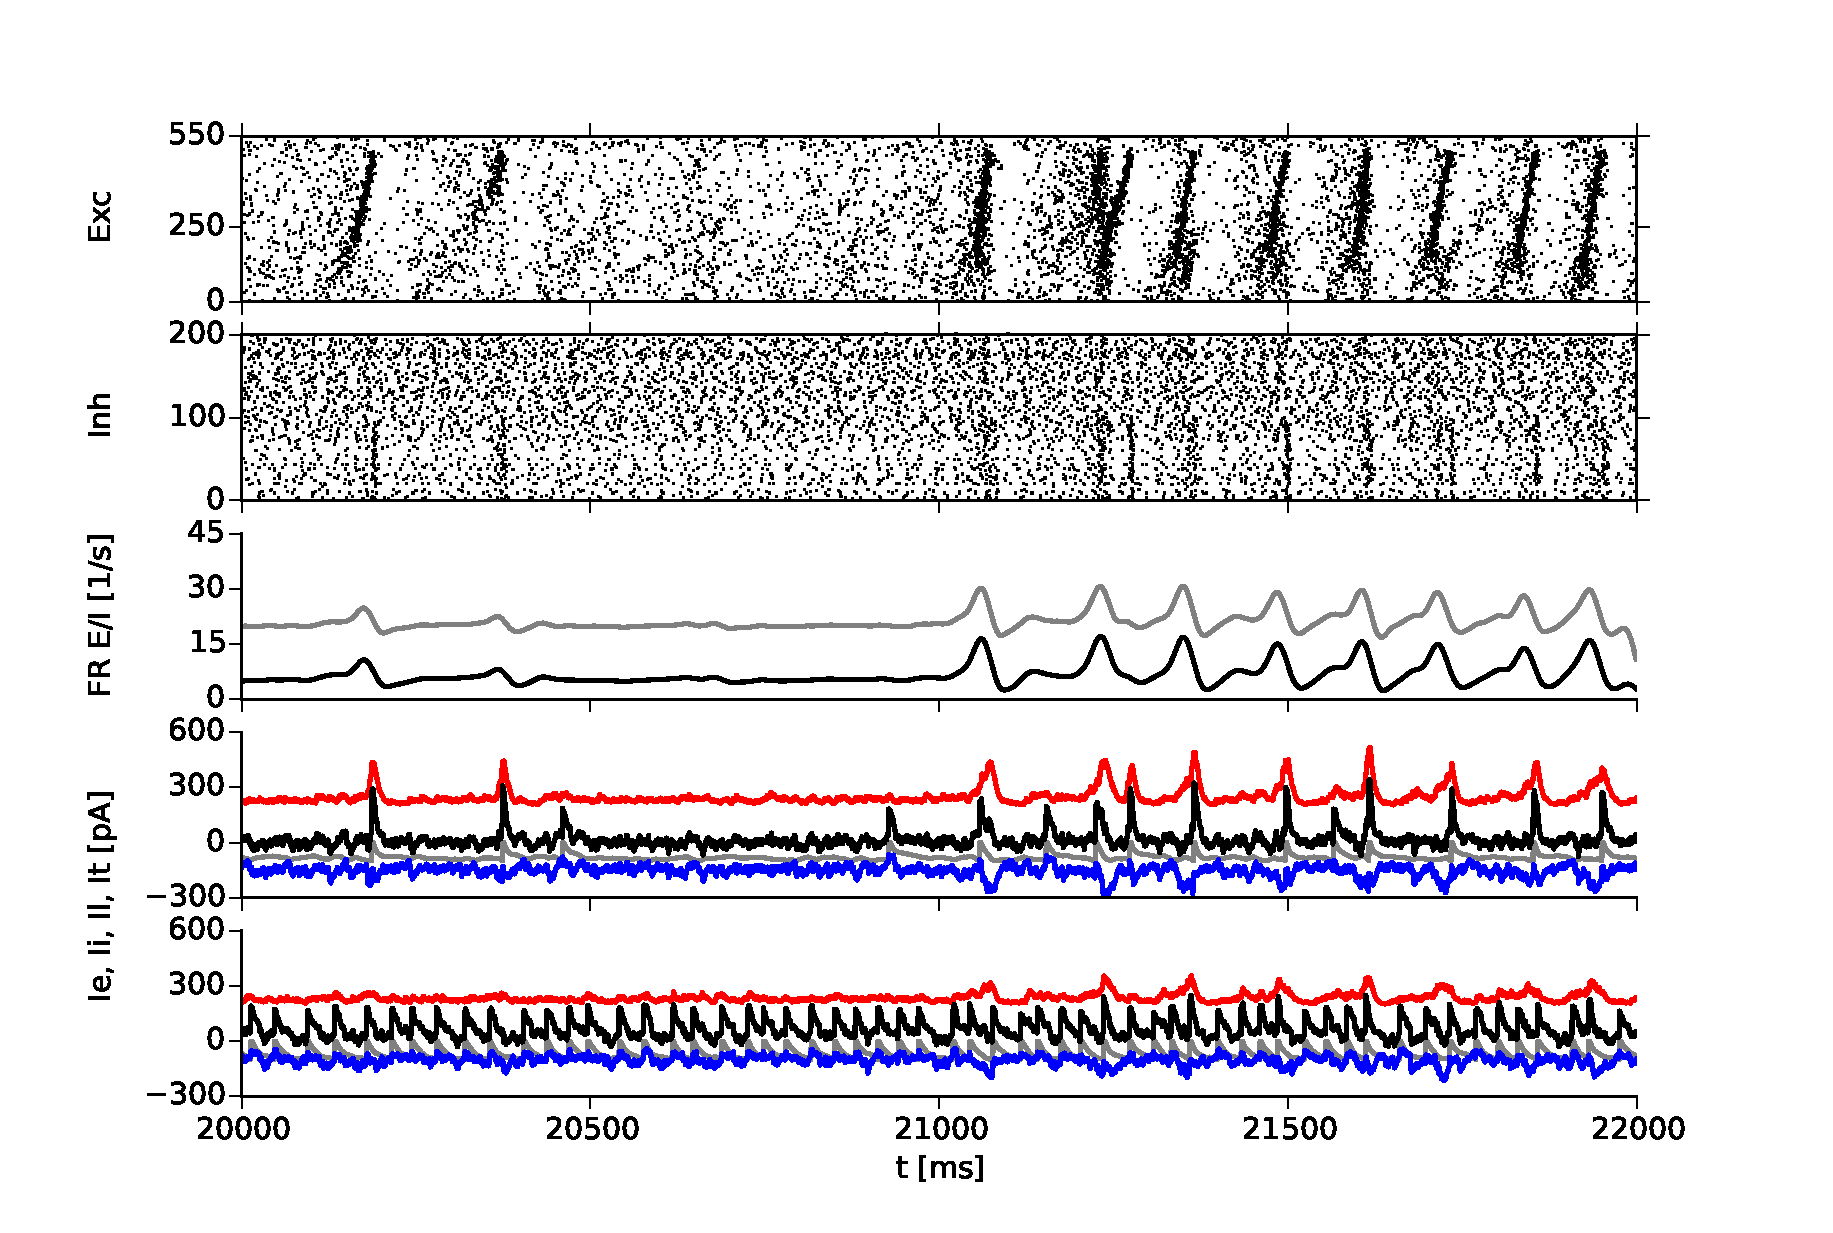
\includegraphics[width =35pc]{gabazine_sim.eps}
      \caption{Decreasing all inhibitory conductances leads to increase in
                spontaneous replays.
              Decreasing only i-i conductances leads to increase in I fr in
              the case of weak gee}
      \label{fig:gabazine_sim}
    \end{figure}

    So how can we explain the gabazine-associated decrease of SWR incidence?
    One hypothesis is that gabazine has different effects on different synapses
    gabaA synapses are various with different structure and combinations of
    untits. For example tonic gabaAR are gabazine insensitive. Other gA
    synapses show also different affinity to gabazine.
    
    More specifically, if i-to-i synapses are affected to a larger
    degree than the i-to-e synapses, one could expect a network that is less
    disinhibited and thus the excitatory population receives more inhibition
    resulting in smaller firing rates. 

    As a toy example, I consider the limiting case where gabazine affects
    i-to-i synapses only in our simulations.  Intuitively expected results are
    I rate goes up because of the smaller self-inhibition due to drug
    application and as a result the E rate goes down. See Figure:

    \begin{figure}
      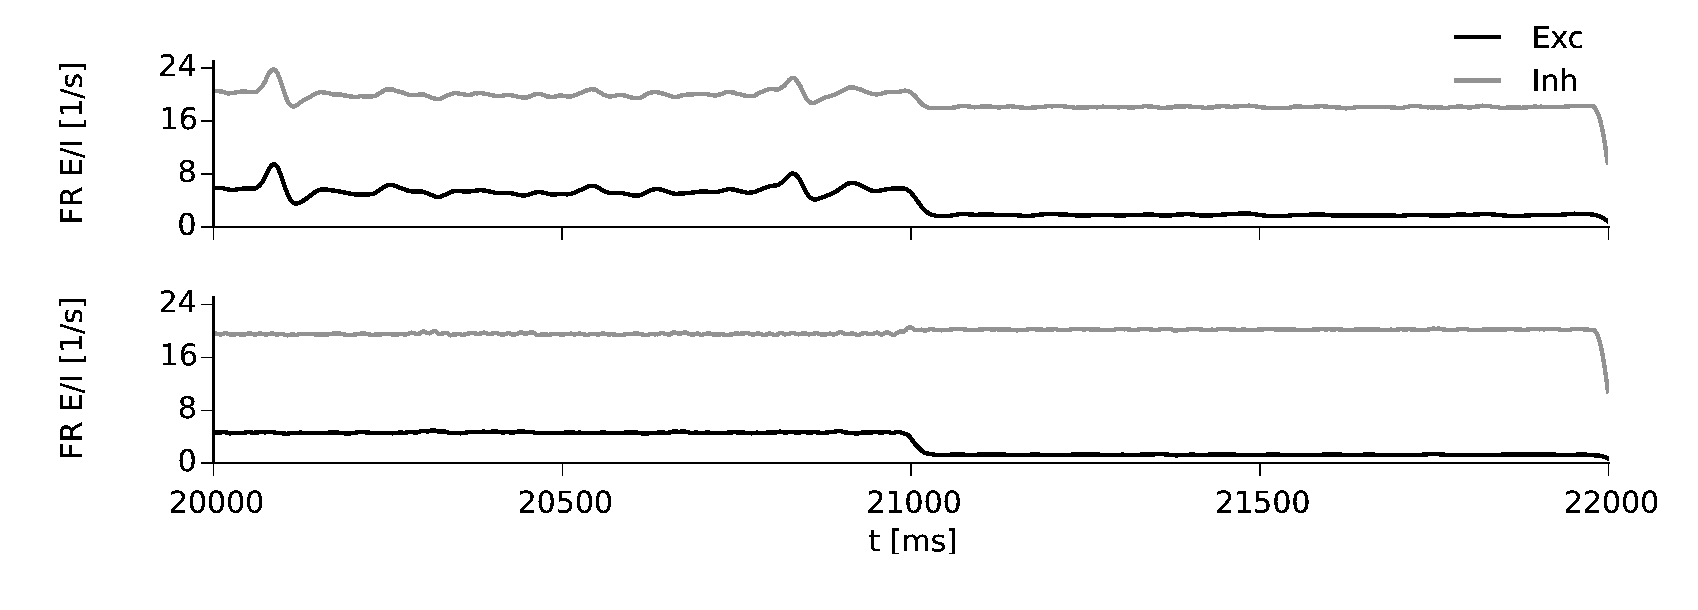
\includegraphics[width =35pc]{gabazine_sim_gii.eps}
      \caption{Decreasing only i-i conductances leads to decrease of both e and
                i FR and of spontaneous replays as well}
      \label{fig:gabazine_sim_giionly}
    \end{figure}
    
    Surprisingly, while decreasing both i-to-i conductances only, we see
    decrease in FR of both e and i populations ref. How does it happen that E
    neurons receiving weaker inhibitory input, fire less? To capture the
    dynamics of the rate change I apply a linear model of a balanced network
    and analyse how the frs depend on the gabazine.

    \begin{equation}
      \begin{split}
        \tau \frac{\text{d}r^E}{\text{d}t} &= - r^E + w_{\rm ee} \, r^E -w_{\rm ei} \, r^I + I_e\\
        \tau \frac{\text{d}r^I}{\text{d}t} &= - r^I + w_{\rm ie} \, r^E -w_{\rm ii} \, r^I + I_i . \\
      \end{split}
      \label{eq:balanced_net}
    \end{equation}

    here re and ri are E.i frs while wxy is the connection weight between y and x (x,y=e,i). tau is tau, I..

    Assuming that we are in a balanced network and in a steady state, then the
    rates do not change, i.e., $ \frac{\text{d}r^I}{\text{d}t} = 0$ and
    $\frac{\text{d}r^I}{\text{d}t} = 0 $.  The stationary solution is then:

    \begin{equation}
      \begin{split}
        r^E &= \frac{(1+w_{\rm ii} - w_{\rm ei})}{w_{\rm ie}w_{\rm ei} - (1+w_{\rm ii})(-1+w_{\rm ee})} I_0 \\
        r^I &= \frac{(1+w_{\rm ie} - w_{\rm ee})}{w_{\rm ie}w_{\rm ei} - (1+w_{\rm ii})(-1+w_{\rm ee})} I_0
      \end{split}
      \label{eq:balanced_sol}
    \end{equation}
  
    To understand how gabazine-induced decrease of gii connections affects the
    firing rate, I can look at how do the steady-state FRs depend on wii:

    \begin{equation}
      \begin{split}
        \frac{\partial r^E}{\partial w_{\rm ii}} &= I_0 \frac{w_{\rm ei} (1 + w_{\rm ie} - w_{\rm ee})} {D^2} \\
        \frac{\partial r^I}{\partial w_{\rm ii}} &= I_0 \frac{(-1 + w_{\rm ee})(1 + w_{\rm ie} - w_{\rm ee})} {D^2} \\
      \end{split}
      \label{eq:drdwii}
    \end{equation}
  
    \begin{equation}
      \begin{split}
        \frac{\partial r^E}{\partial w_{\rm ei}} &= I_0 \frac{-(1 + w_{\rm ii}) (1 + w_{\rm ie} - w_{\rm ee})} {D^2} \\
        \frac{\partial r^I}{\partial w_{\rm ei}} &= I_0 \frac{-w_{\rm ie} (1 + w_{\rm ie} - w_{\rm ee})} {D^2} \\
      \end{split}
      \label{eq:drdwei}
    \end{equation}


    \[
      \frac{\partial r^E}{\partial w_{\rm ei}} + \frac{\partial r^E}{\partial w_{\rm ii}} =  I_0 \frac{(-1 - w_{\rm ii} + w_{\rm ei}) (1 + w_{\rm ie} - w_{\rm ee})} {D^2} 
    \]

    \[
      \frac{\partial r^I}{\partial w_{\rm ei}} + \frac{\partial r^I}{\partial w_{\rm ii}} =  I_0 \frac{- (1 + w_{\rm ie} - w_{\rm ee})^2} {D^2} 
    \]

    Assuming that the inhibitory and excitatory input weights are similar,
    i.e., $1 - w_{\rm xe} + w_{\rm xi} > 0$ on both excitatory and inhibitory
    neurons ($x=e,i$). then re would have positive derivative in respect to wii
    (with some additional condit.?). Meaning that a decrease in wii would lead
    to decrease in re. which is intuitive. The inhibitory firing, however,
    depends heavily on the e-to-e weights. If wee>1, then dri dwii is positive,
    meaning that I fr will decrease after the gabazine application. This is the
    scenario that we see in the simulation in Figure
    \ref{fig:gabazine_sim_giionly}.

    To test the validity of this calculation, here are the results of the
    simulated gabazine in a network with weaker gee (5-fold weaker than the
    original simulation). We see that in the case of weak gee, the inhibitory
    fr increases indeed when gabazine is presented (Figure x)

    state the hypothesis of Gb controlling the incidence...after a big event
    larger hyperpolarisation..alternative different effects of gabazine on i-i
    and i-e synapses?

  \subsection{GabaB antagonist increases SWR incidence}
    To answer what modulates the incidence of SWs we need a time constant of
    the same magnitude as the interval between events. A potential candidate is
    the gBR which operates on the time scale of hundreds of milliseconds (ref).
    Here I test the properties of network dynamics measured with an
    extracellular electrode after a gB antagonist is infused into a slice.

    gB has been shown to be involved in SW modulation, but also Behrens? showed
    that in their model it did not modulate incidence?  Here we analysed 13?
    recordings where baseline activity was measured and then SCH was infused
    Fig here.

      \begin{figure}
        \includegraphics[width =35pc]{19march13_slice1.png}
        \caption{ Example recording. GabaB antagonist increases SWR incidence 
                }
      \end{figure}

    gB increased SWR incidence: pooled (incidence, peak, duration)
    gB has a relative fast effect \~ 3 mins.
    discuss possible binding sides, possible effects?
    nikolaus's paper on cannabinoids checked pre/postsynaptic effects... 

    \begin{figure}
    \includegraphics[width =35pc]{SCH_all.eps}
    \caption{GB antagonist pooled
              Bottom: mean values before the drug is infused (from -5 to 0 mins), and after (from 2-7 mins)
            }
    \end{figure}
    
    However, seems not to be crucial for SWRs, but only facilitates a bit?
    here a figure of inicid before vs. incid after!

    discuss possible gBR locations

  \subsection{Looking for postsynaptic GB affects}

    SW detection and associated Vm in a patched PC.
    Note that there are number of EPSPs (compound) outside of events.
    However, IPSPs are rare. They mostly come during population events, SWs or
    some other smaller events that are not necessary SWs, e.g., inhibiory
    unitary potentyial (Bazselot 2010).
    \begin{figure}
      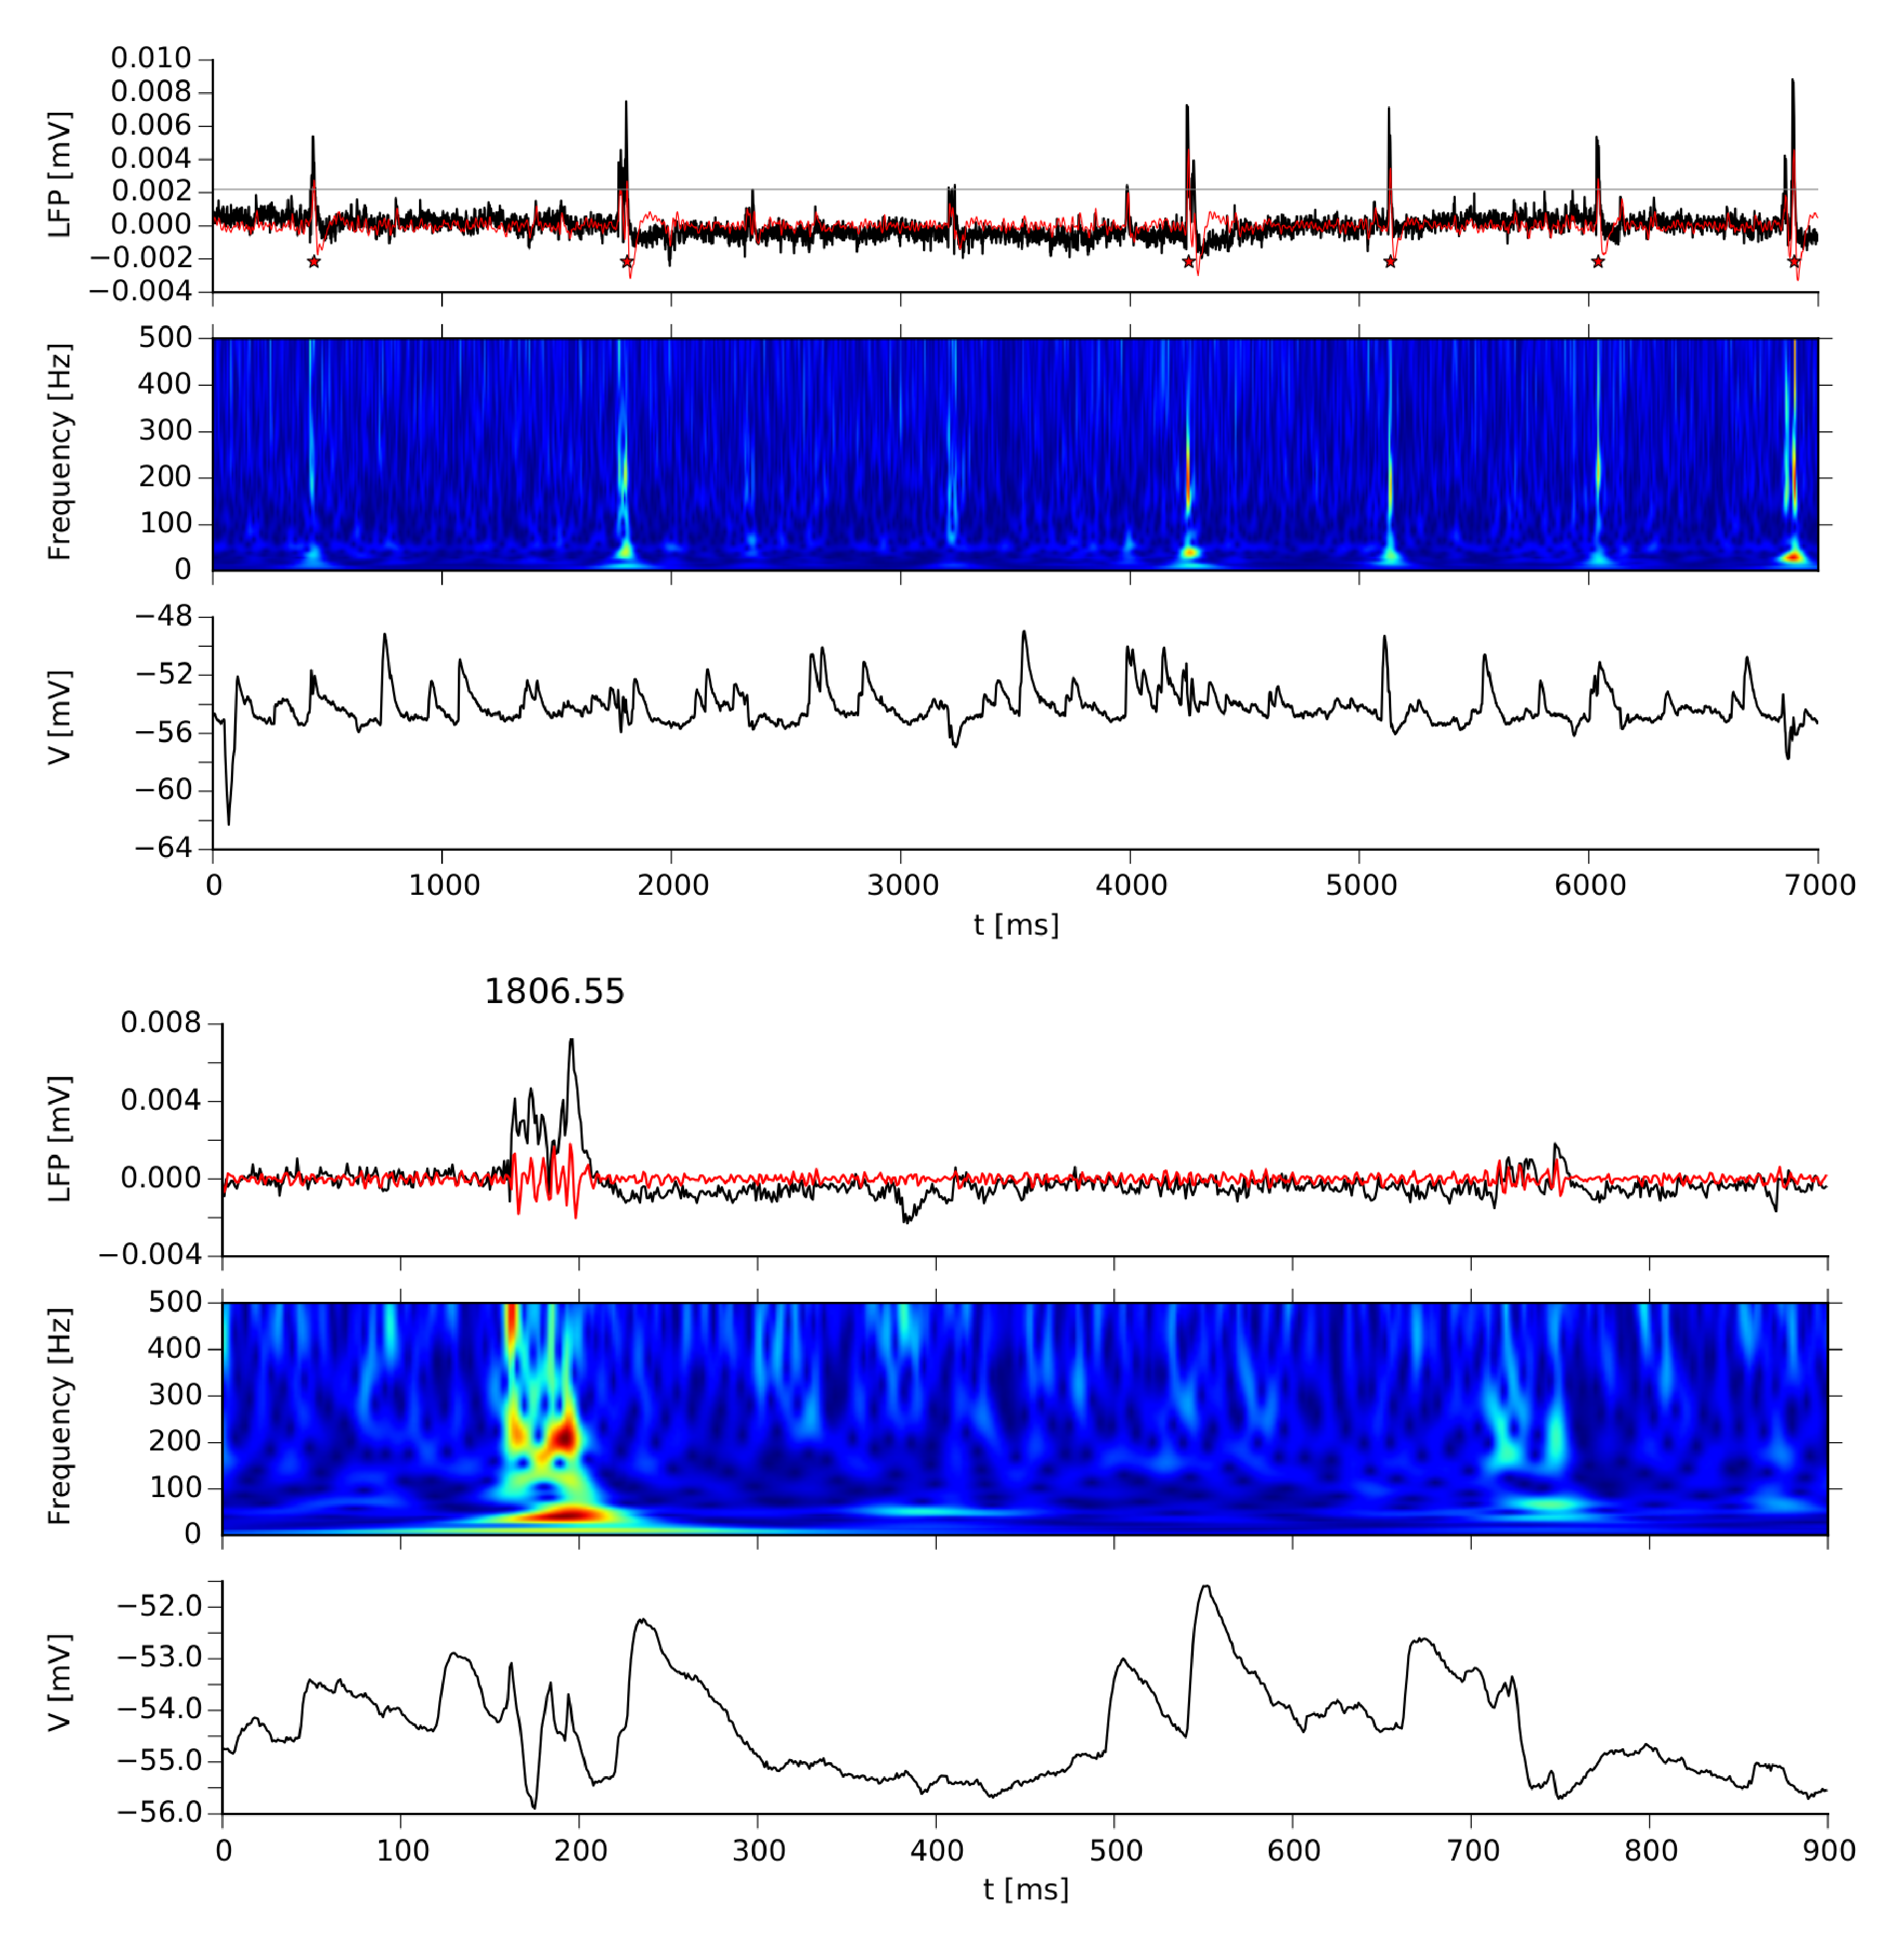
\includegraphics[width =35pc]{intra_example.eps}
      \caption{ Example recording. SWR detection, corresponding intra recording...
              }
    \end{figure}

    one example (the only one) where we can observe fast and slow
    hyperpolarisation during SW events. 
    \begin{figure}
      \includegraphics[width =35pc]{14jan11_cell1_xxx.pdf}
      \caption{ Example recording. simultaneous extra/intra recordings. 
        intra-recordings overlayed, and averaged...
              }
    \end{figure}

    mean SW-associated Vms:
    \begin{figure}
      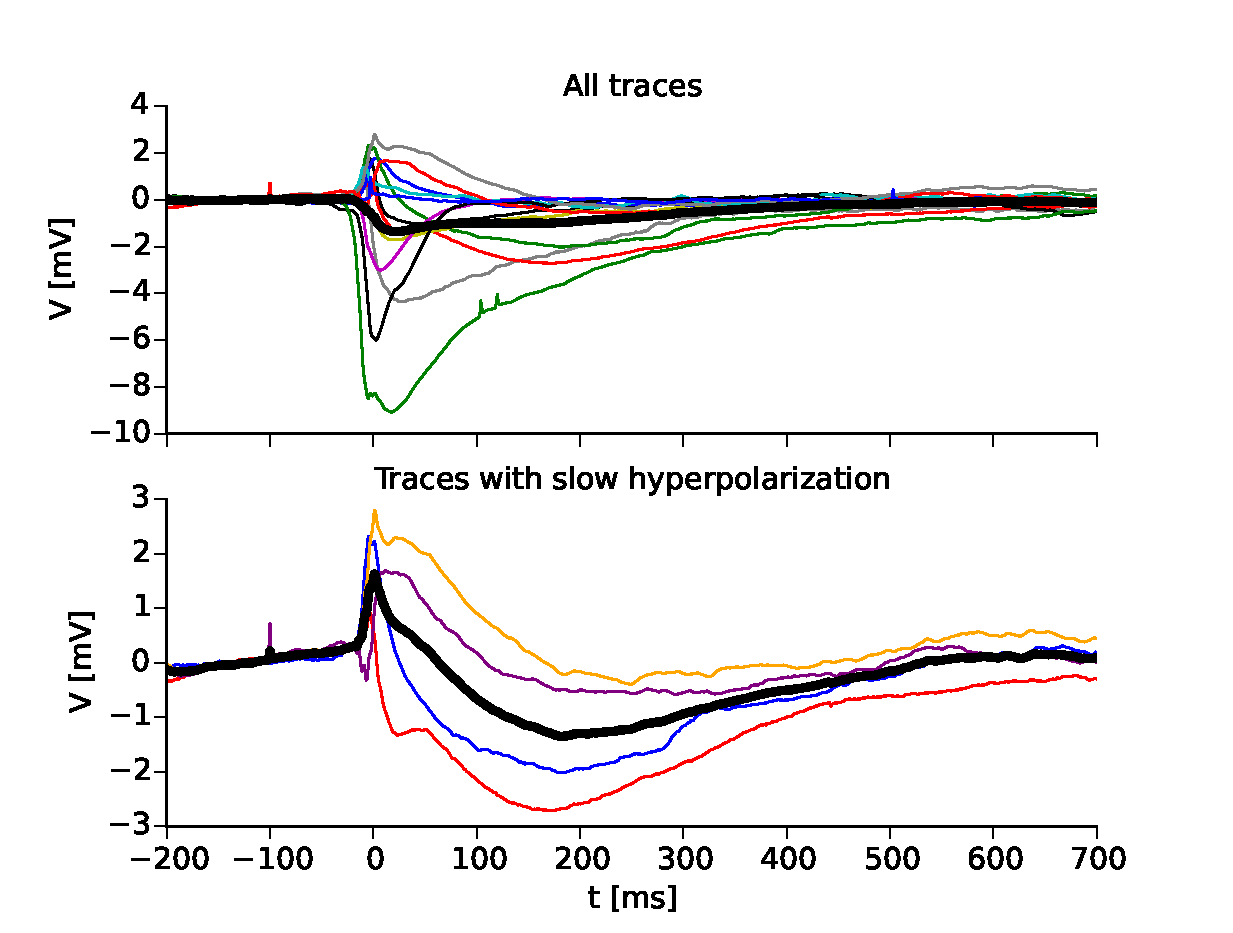
\includegraphics[width =35pc]{mean_intras.eps}
      \caption{ Mean SW-associated voltage traces for each cell is in color;
        black line is the mean of the means. bottom: mean voltage traces of
        cells that show slow, possibly gB-evoked hyperpolarization. all
        traces are normalized by subtracting the mean potential in the before
        the event.
              }
    \end{figure}

    Larger events evoke stronger hyperpolarizastion in every cell that gets hyperpolarised after an event.
    iSWi is however not consistently related with any intracellular responses...

      \begin{figure}
        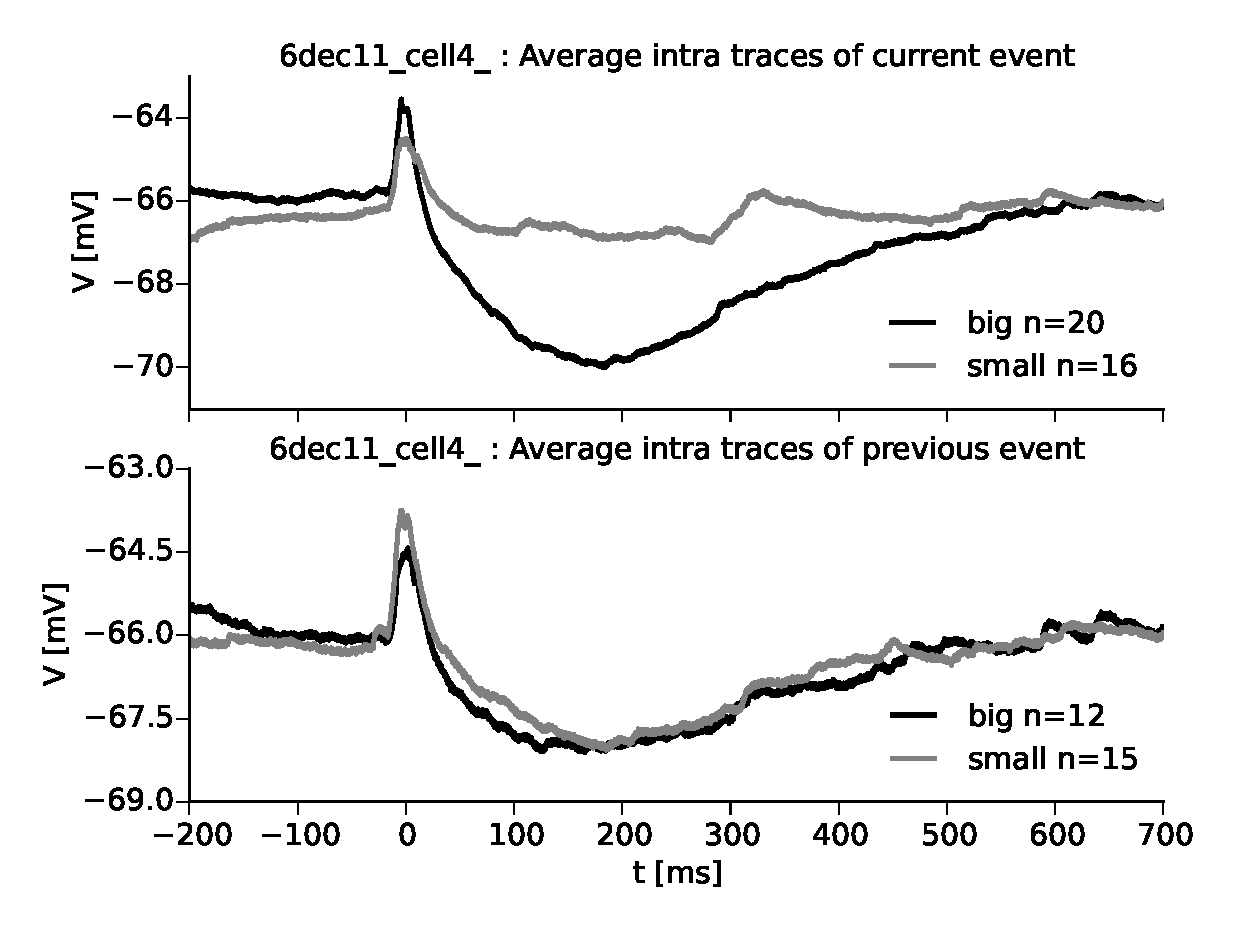
\includegraphics[width =35pc]{6dec11_cell4_000.eps}
        \caption{ Example recording. Big events are associated with a larger
          hyperpolarisation (top). Here smaller events (30\% of the smallest
          SWs) did not evoke gB-associated response. Bottom: there is no
          correlation between the depolarisation of a cell and the size of the
          following event.
                }
      \end{figure}
    
    ref to gB review that I have printed, show a figure(s) from there

    from dataset3 (former dataset 1): intra/extra

    6/13 got fast hyperpolarisation
    4/13 got slow gB component.
    1/13 got slow and fast components
    1,2/13 no hyp..to noisy or..
    8/14 got transient depolarisation during events 

    gB polarisation is correlated with the size of events

    gB response is not correlated with the interval till next event, which is an evidence against the hypothesis proposed above
    (check Hulse for comparison of results)

    extrasynaptic gB receptors?
    presynaptic?
    simultaneous gabazine and gB antagonist might shed some light?

    show single recording example and pooled from all.

    slight depolarisation in each cell before SWs..mean of gB cells

  \subsection{serial correlations between SWR events}

    \begin{figure}
      \includegraphics[width= 30pc]{ca3only-cs.eps}
      \caption{
        Serial correlation of spontaneous ca3 SWs.
             }
      \label{fig:ca3only_SCsumm}
    \end{figure}

    \begin{figure}
      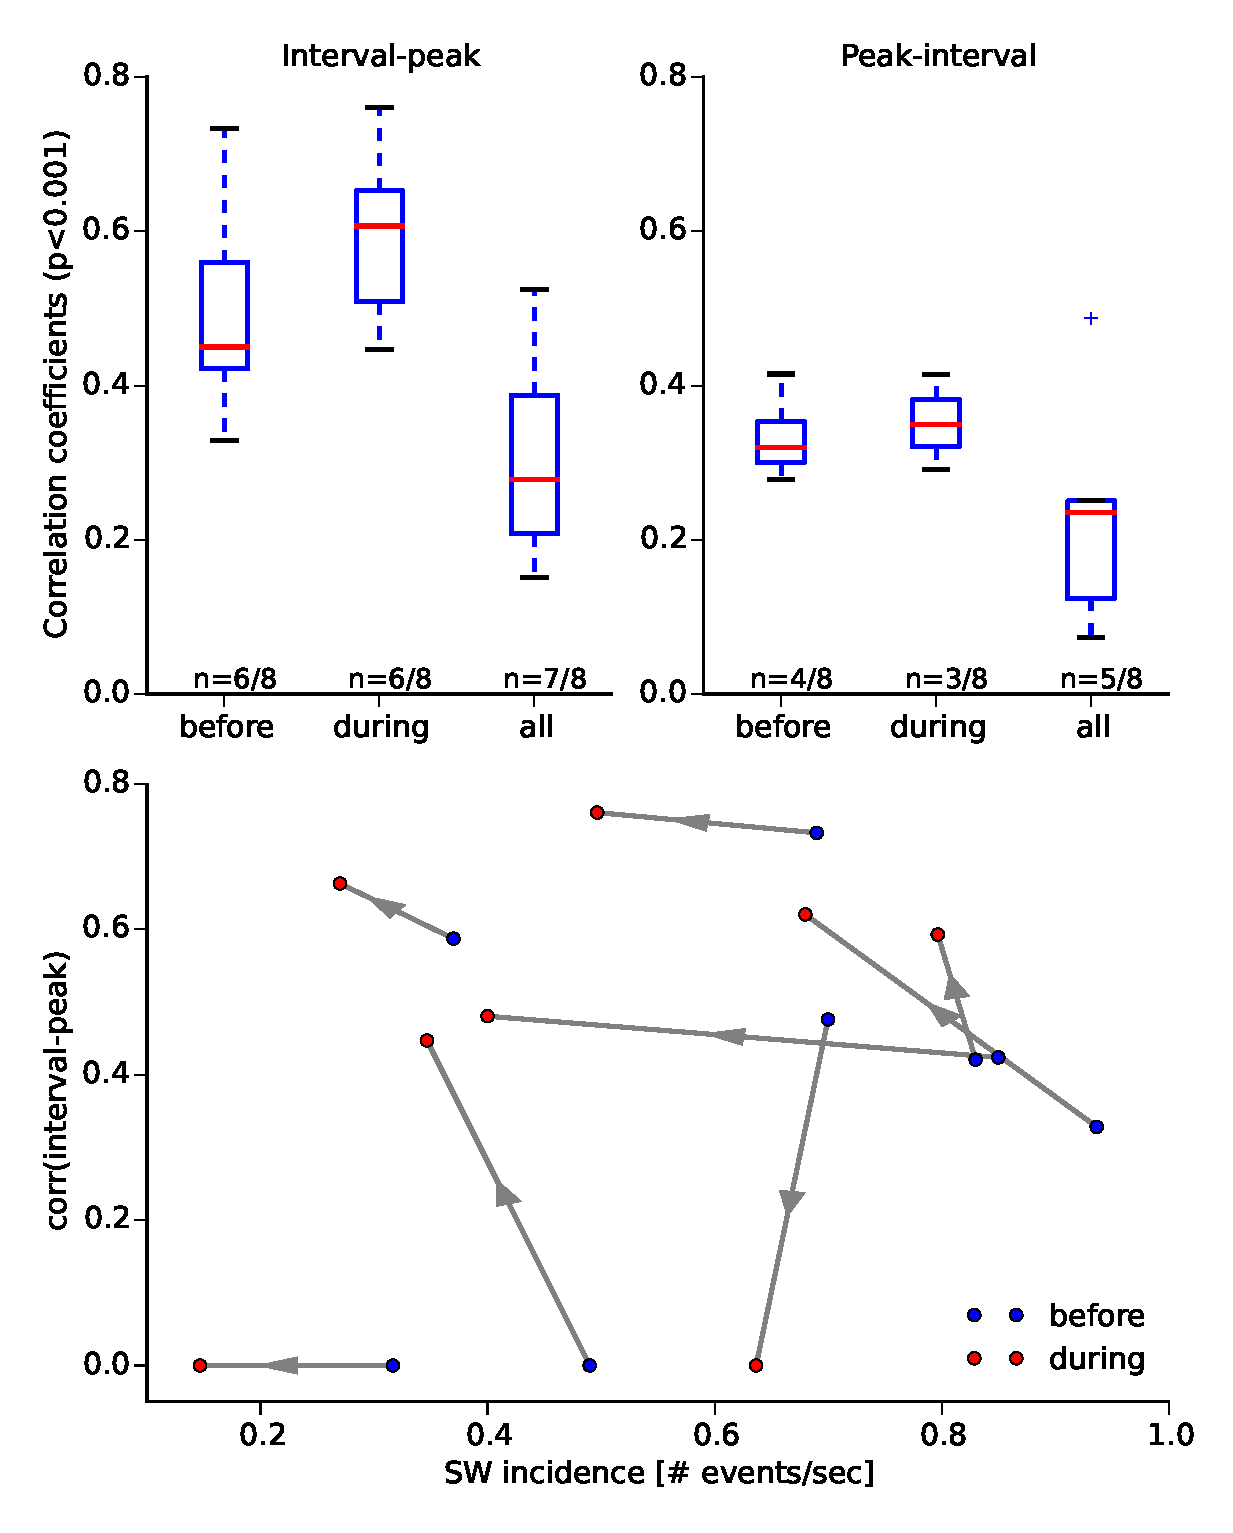
\includegraphics[width= 30pc]{gabazine_SCsumm.eps}
      \caption{
        Serial correlation before during gabazine. SC and incidence relation.
             }
      \label{fig:gabazine_SCsumm}
    \end{figure}

    \begin{figure}
      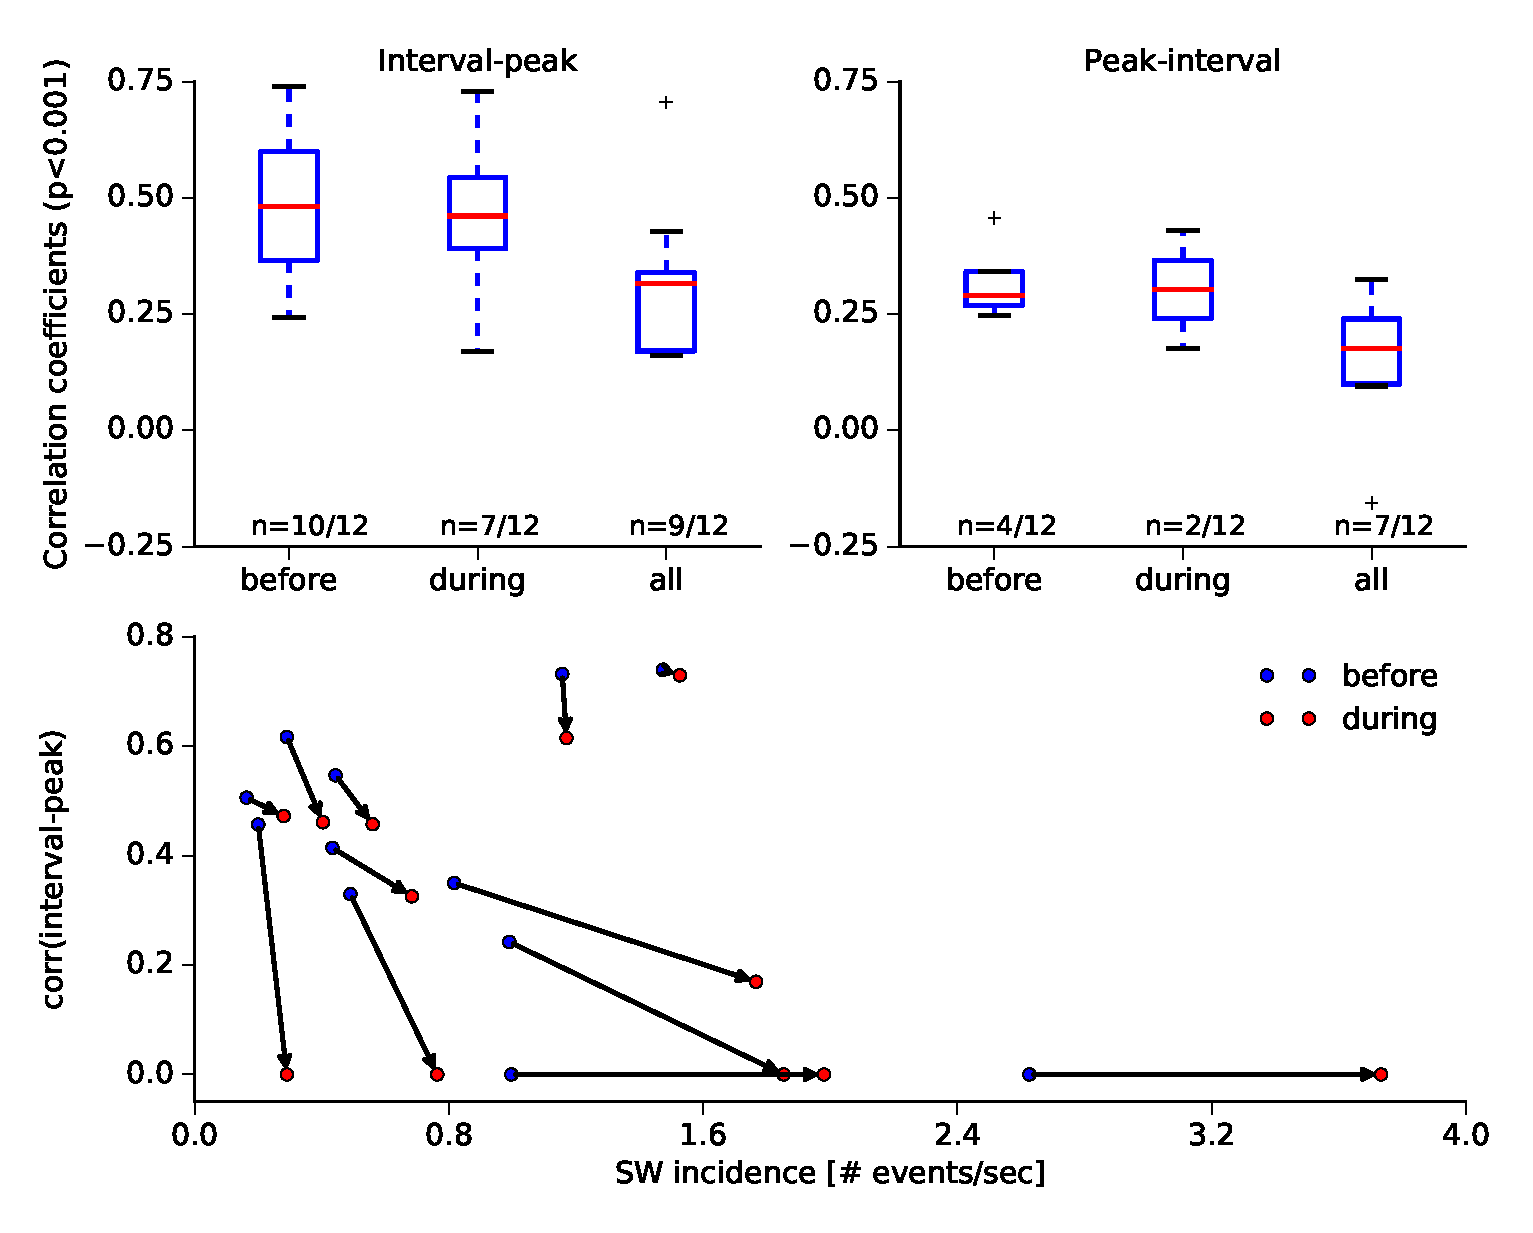
\includegraphics[width= 30pc]{SCH_SCsumm.eps}
      \caption{
        Serial correlation before during GabaB antagonist. SC and incidence relation.
             }
      \label{fig:SCH_SCsumm}
    \end{figure}

    If its the gaba spillover that controls the interval, then after a big wave
    there will be a bigger spillover and thus a bigger interval till next
    event..This argument is for pre/post/extra-synaptic GB A and B receptors?

    expected serial correlations: peak-iSWi was not found but iSWi-peak instead.
    from dataset4 (former dataset 3): CA3 extracellular only
    summary whisker figure of all SCs (dataset 3) ii and aa as well!


    note the relatively weak a-i correlation
    discuss the much high i-a correlation (ref Kohus that replicated our
    finding :)). Some recovery that does not necessary depend on the size of
    the event?  or possible multiple initiation zones and therefore no chance
    to ai correlations

    serial correlations with drugs (gabzine/sch and incidence) 

  \subsection{where is the SWa-iSWi correlation}

    \begin{figure}
      \includegraphics[width= 35pc]{D_141126_s08_0003.eps}
      \caption{
        An example of the MEA configuration and location on the hp slice.  The
        colored channels are recording..  Example of a recording sweep where
        SWR peaks measured at different electrodes are plotted in time. Here
        for each recording site, the peaks are normalized to 0 mean and std of
        1 for better comparison
      }
      \label{fig:peak_correlation_ex}
    \end{figure}

    A possible explanation for the missing peak-interval correlations is that
    the SW amplitude is measured at a particular location at the slice, and
    this location might not be the representative of what is going on in the
    slice. hypothesis: SWs occur at different locations in the slice and
    propagate through the CA3 area in various directions. It is possible that a
    particular event might look big at one location but weak at another.
    Therefore, in the single electrode recordings, we can't say anything about
    the next occurrence based on the measured amplitude, as SW can originate
    elsewhere and the local depletion recovery doesn't play any role in
    controlling the event. 

    here results from all MAE data. 

    \begin{figure}
      \includegraphics[width= 25pc]{mea_corrs_summ.eps}
      \caption{
              Distribution of correlations between SWR peaks measured at
              different locations in the hp
             }
      \label{fig:peak_correlation_ex}
    \end{figure}

    estimate of 2116 pairs of channels. all correlations are plotted in Fig x
    and all correlation are significant with p<0.001

    Seems it's not the case that SWs have very different amplitudes at
    different location. Of course the mea covers only limited surface of the hp
    and Sw might still originate elsewhere. For example there are indication
    that SWs can be originating in subiculum and just then propagate to ca3.
    such origin of the SW would leave no chance for descent AI correlations to
    manifest themselves. One way is to isolate external influence of the ca3,
    and this can be achieved by using ca3 minislices in which we know swrs can
    manifest themselves.


\section{Discussion}
  alternative hypothesis: presynaptic gB, see Nikolaus canabonoid paper supplementary
  consequences of such prediction. 
  disinhibitory trigger for SWR???

  possible that PCs cells receive only EPSP without from spontaneous synaptic
  release, and those built up in time until network bursts in a SW..Then how to
  explain PVBC activation leads to SW... shallow IPSP from the balancing INs,
  possibly targetting the distal branches of the dentrites?

  \subsection{Hypothesis on how gabazine affects SWR incidence} 

    It has been show that gabazine, which is a ${\rm GABA_A}$ receptor
    antagonist, leads to lower incidence of SWRs. It is unclear why a reduction
    of inhibition leads to a reduction of SWR incidence, which is
    counterintuitive.

    In simulations of balanced networks we use the assembly sequence as a model
    for the SWR phenomenon that can spontaneously occur. As intuitively
    expected, decreasing all inhibitory conductances (with $\sim 5 \%$) leads
    to an increase of spontaneous replay incidence. However, a differentiated
    role of gabazine on the I-to-E and I-to-I synapses in our simulation could
    replicate the original gabazine experiment. More specifically, if I-to-I
    synapses are affected to a larger degree than the I-to-E synapses, then the
    incidence of spontaneous bursts is decreased. Can this indeed be an
    explanation of the gabazine associated decrease of SWRs is to be
    discovered?

    figure on simulated gabazine..how to look exactly..raster plots where one sees bursts?? 2 subfigures with exp decreasing inh conductances..same and diff rate for ei and ii

    A possible experiment can be conducted to test the validity of such
    hypothesis.  Pairs of presynaptic IN (e.g. PVBC) and a postsynaptic cell
    (PC or IN) is to be found.  The postsynaptic cell is patched while the
    presynaptic cell is driven to fire and IPSPs are measured.  The same
    stimulation is applied again after the infusion of gabazine in the slice
    and IPSP are detected.  The effects of gabazine should be observable in
    both I-to-E and I-to-I synapses, e.g., IPSPs are decreased.  However, a
    stronger decrease due to the drug application is to be expected on the
    I-to-I synapses than on i-to-e synapses.

    Alternatively to the aforementioned hypothesis, another explanation might
    be the fact that gabazine application simply increases the firing rate of
    INs \citep{Schlingloff2014}, and the increased IN firing leads to more
    release of GABA which can activate extrasynaptic GABAR on PC (GABAa or b)
    that inhibit the pyramids and IN as well. As extrasynaptic effects are slow
    this leads to increased iSWis. To test this hypothesis should be easier. In
    the presence of extrasynaptic blockers (GB blocker, or tonic GA
    antagonist), SWR incidence is measured. Then, the application of gabazine
    should not lead to increase of the iSWi.  As we have seen in the analysed
    data, GBr do not seem to have a strong presence on the postsynaptic side of
    PCs. maybe pre/extrasynaptic gB can be disentangled? Alternatively, gB on
    i-to-i presynaptic side?  However the lack of peak-interval correlation
    speaks against this hypothesis..

    A differential short-term depression of I-to-E and I-to-I synapses could
    also explain the observed correlation between SWR amplitude and the
    following interval to the next SWR. For simplicity we neglect short-term
    depression of I-to-E synapses. The recovery from depression (after a SWR)
    of I-to-I synapses (Kohus et al., 2016) increases these synapses with a
    time constant on the order of hundreds of milliseconds. As a result, the
    activity of the inhibitory neurons gradually decreases, which in turn
    reduces the inhibition onto pyramidal cells. Pyramidal cells in CA3 slowly
    increase their activity long before a SWR (de la Prida 2006; Schlingloff,
    2014; Hulse et al, 2016) until some critical activity level is reached
    where additional fluctuations/noise can trigger a new SWR.  If depression
    was the cause, then larger waves would give rise to larger depression, and
    therefore, to longer interval until next event.

    Prediction for experiments: ...

    possible virus that can be injected in PVBC (or other PVIN) and that spreads to postsynaptic cells, and stains them. Then one can see to what kind of INs do the PVINs project to and try to find the ones that might be disinhibited for the SW onset.

  \subsection{Hypothesis on how GABA affects on SWR incidence} 

    Why, then, does application of GABA to a slice also decrease SWR
    incidence, although this may have the opposite effect compared to
    gabazine? (add some REF)

    In simulations of balanced networks, adding low GABAergic conductances
    to all neurons decreases SWR incidence (TRUE? should be, injecting small inh current did the job).

    To explain the observed effect in slices, we may have to add to the
    picture the extrasynaptic $GABA_A$ receptors (tonic GABA)... maybe also
    $GABA_B$ (?).  We assume that the default state in a slice is that they
    are closed (is that true?), and therefore gabazine cannot change their
    conductance. In contrast, adding GABA to the slice activates these
    extrasynaptic receptors, which have a quite low affinity to GABA
    compared to intrasynaptic GABAA receptors (to be checked!). As a
    result, appliation of GABA hyperpolarizes cells or acts shunting, and
    thus stongly reduces the activity of pyramids, which decreases or
    abolishes SWRs.

    Prediction for experiments: ...

    A fact: gabazine decreases the multi unit activity during SWRs measured with a tetrode.b
    However, applying loose-patch to PVBC reveals that they actually increase their firing rate
    when gabazine is infused in the slice. Therefore, gabazine decreases the excitability of the
    whole network and increases the firing PVBC and possibly also of other INs (Schlingloff, 2014).
    Therefore gabazine actually increases gaba levels...



\section{todo}


%###################
Concrete shit only:
%###################
new serial corr figure (ca3 only)

- lit on FRs of INs adter drugs..gabazine SCH
- on Figures of SC and incidence, put some arrows
- gB antagonist; is there effect like Nikolaus showed; low incidence, higher influence; change the intervals a bit!
- linear model/ same or diff curr?
- extra plot of ri increasing/decreasing
- new fig on SCH incidence modulation; peak and duration of all data
- include gB simulation; explain how we do it..equations in pres.pdf in Nikolaus 1 folder


literature:
check vida's studies!
- check gabazine literature
  - effects, e.g. gabaA blocker?
  - prev studies of gabazine on SWs
  - literature on gabaA channs, gating units and gabazine binding efficacies to them??
  - 

literature facts to add:

- schlingloff:
    - ..blocking exc inputs still makes SWRs but smaller!!
    - Question: why there are still few ripples after the offset of a brief light stimulation in the absence of Exc transmission? IN GJ?

- ellender:
            - for SW initiation: cut DG from CA3 has no effect on incidence
            - cut ca3 from ca1, no SWs in CA1, therefore CA3 is the initiation zone
            - arise locally and independently in all ca3 subregions
            - also PY FR probability slightly increases before SW
            - various drugs for SW generation: to check!
            - An individual perisomatic-targeting interneuron can suppress and subsequently enhance sharp wave incidence
            - PTI activation (depolarized for 500 ms) have imidiate suppression effect and then enhancement effect in 1-2 secs.
            - The suppression and postinhibitory enhancement of sharp wave generation is local to the axonal arborization of the stimulated perisomatic-targeting interneuron.

- Rasch2007: place-coding odors presented during SW sleep improve memory
- bazelot2010: unitary inhibitory field potential
            - anticorrelated Vm and extracell recording...17feb12cell2  has something like that 
            - single AP in IN evokes monosynaptic LFP response (field IPSPs); single AP of PC evokes disynaptic field IPSPs
            - clusters of LFP activity signitures
            - dendritic vs perisomatic events; slower, faster; infrequent vs frequent; 

- Kohus2016: suggest that the recovery of STD of PVBC is responsible for the iSWi. Why? Because time-constants match? But there are no ipsps visible outside of events, maybe because tonic inhibition comes to distant dendritic branches and therefore are not visible in the patched cells; 17feb12cell2 has double SWs which kind of contradict the min refr period. maybe its 2 subnetworks; echo of a Sw, travelling wave phenomenon...

- Karnanani: disinhibitory circuit in cortex...


- Hulse, Schlinglof, ....

- James, 1890: 

- Takahashi2010: organotopic slices, clustering in CA3, connected cells havew common input, correlated; bidirectional connections, 28.8\% connectivity.

Yeung2003:
  -gabazine: competitive antagonist affects only phasic(synaptic) GABAa channels, not tonic in hippocampal culture! in DG, tonic channels are affected; implies that underlying receptors contain gamma subunit but not delta;

  -Gabaa receptors have multiple binding sides, each with a different affinity to GABA
  -low-conductance opening of GABAa channels are insensitive to gabazine

Lerma et al.: ambient GABA in the brain ~0.2-0.8 uM gaba in the brain

Beato2007: gabazine is antagonist for glycine receptors

Ueno1997: gabazine is allosteric inhibitor of channel openning of gabaa receptors; gbz, BCL are competitive antagonists of GABA binding; for receptors with beta2 subunit steroids could still activate the channel

Christensen2014: method for detecting extrasynaptic gaba with a whole-cell sniffer; resolution of few tens of nM, millisecond time resolution; using human embryonic kidney (HEK) cell line

Maier2003, Nimmrich2005: GBZ (=>1mM) abolishes SWRs 

Maier2012: SWR suppression is not due to postsynaptic effects; GIRK blocker has no effect

Macdonald94: review on GABAaR

knowles84: [gabaBR] early and late IPSPs; late ipsps are gone after the cells is depolarized for a longer time (desensitisation?); likely to be generated in dentrites; as ipsps are relatively insensitive to hyperpolarization of the soma; no late IPSP after prolonged exposure to bicuculline and picrotoxin

%###################
Done Shit here:
%###################
- math: all conditions in simulated gabazine analytical model...compare to simulations..
- for average gabazine plot, take as a baseline the incidence in [-17,0] mins
- plot of intra trace only to highlight the constant bombardment with epsp 
- count/ quantify hyperpolar in extra/intra dataset..
- 1 figure with the different mean gb responces from intra?
- plot in py fig some of the intra recordings to see if there is really an effect, e.g.: 17feb12 (1, 4 and 5)
- summary whisker plot figure for all SCs in dataset3 
- figure gB antagonist effects: before vs. during. on correlations?
- figure gabazine effects: before vs. during. on correlations?
- for the mea correlation, make some kind of statistic of how significant are all these correlations.: all p values are smaller than 0.001!!!!!!!!!!!
- combine figs of simulated gabazine and show FRs only; put legend
- combine 3.9 and 3.10 and make a new figure only with FRs
- edit 3.5: increase CC subplot; chans; remove CC value from the top; combine it with 3.4 ?????
- Schilinglof, the gabazine experiments make a figure from 2 experiments from the paper

%###################
considered and cancelled
%###################
- f 3.8 individual traces to be made gray; or like an imshow the traces from single events

%###################
good to be done eventually:
%###################
- mea recordings, normalize during each event; see if different sites covary? if events are very close temporary, do they anti-covary


%###################
old unspecified shit is boiling at the bottom:
%###################


pool in various ways

  - take all traces with no drugs...
    - serial correlations
    - kk

literature of gabazine on SWRs


ps theta modulated

disinhibition

open questions:
contributions to LFP during SWRs: synaptic, spiking, inhibitory synapses and spiking?

put an extra Inh population (something like Jose's) to make ripples in the continuous AS?


  according to the hypothesis we would expect:
    - after big events, larger hyperpolarisation.
    - that big events are followed by longer iSWi
    - large gB hyperpolarisation would correlate with long iSWi following the event

